Широкое распространение на практике получили стационарные решения уравнения фильтрации. Приведем некоторые из них.

\subsection{Решение для постоянного давления на круговой границе}

Рассматривается самая простая модель работы добывающей скважины - радиальная стационарная фильтрация в однородном изотропном пласте круговой формы. Скважина находится в центре пласта (рис. \ref{ris:radial_inflow_steady_state_1}). На границе пласта поддерживается постоянное давление. Фактически это означает, что через границу пласта идет поток жидкости, уравновешивающий дебит скважины. 

Решение можно получить как решения уравнения фильтрации, учитывая стационарность потока

\begin{equation} \label{eq:diff_eq_1} 
	\frac{\partial ^2 p }{\partial r^2} + \frac{1}{r} \frac{\partial p}{\partial r} = 0
\end{equation}

  

\begin{figure}[h!]
	\begin{center}
		

\tikzset{every picture/.style={line width=0.75pt}} %set default line width to 0.75pt        

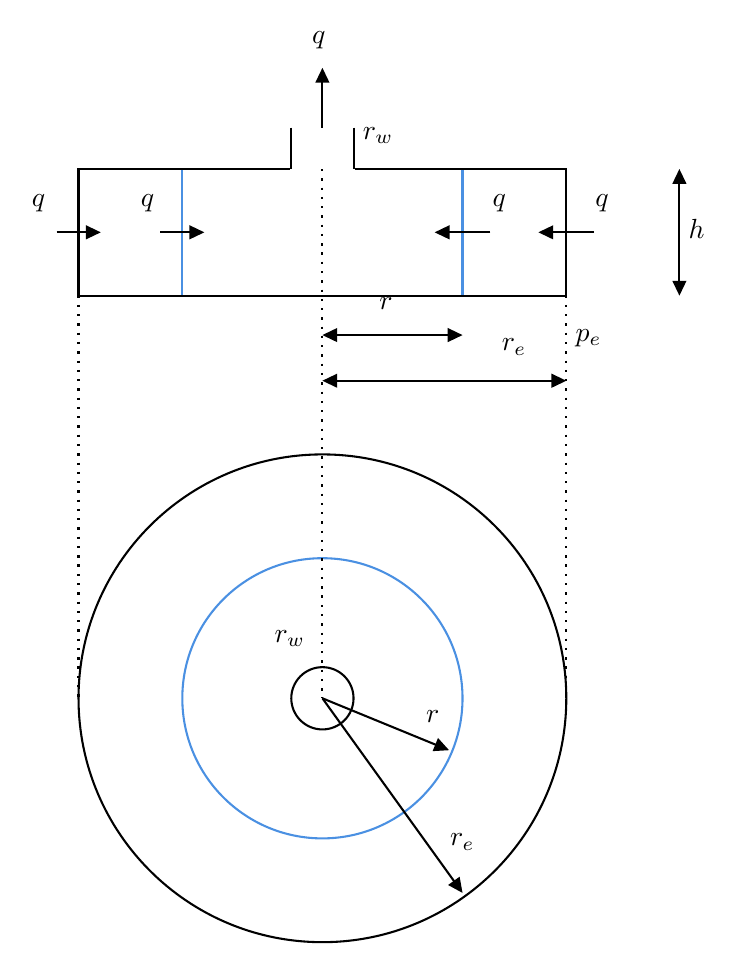
\begin{tikzpicture}[x=0.75pt,y=0.75pt,yscale=-1,xscale=1]
%uncomment if require: \path (0,493); %set diagram left start at 0, and has height of 493

%Shape: Rectangle [id:dp2210940442519349] 
\draw  [color={rgb, 255:red, 74; green, 144; blue, 226 }  ,draw opacity=1 ] (297.5,90) -- (432.5,90) -- (432.5,151) -- (297.5,151) -- cycle ;
%Shape: Circle [id:dp04970297189708517] 
\draw  [color={rgb, 255:red, 74; green, 144; blue, 226 }  ,draw opacity=1 ][fill={rgb, 255:red, 255; green, 255; blue, 255 }  ,fill opacity=1 ] (297.5,345) .. controls (297.5,307.72) and (327.72,277.5) .. (365,277.5) .. controls (402.28,277.5) and (432.5,307.72) .. (432.5,345) .. controls (432.5,382.28) and (402.28,412.5) .. (365,412.5) .. controls (327.72,412.5) and (297.5,382.28) .. (297.5,345) -- cycle ;
%Shape: Circle [id:dp10293196217835776] 
\draw   (247.5,345) .. controls (247.5,280.11) and (300.11,227.5) .. (365,227.5) .. controls (429.89,227.5) and (482.5,280.11) .. (482.5,345) .. controls (482.5,409.89) and (429.89,462.5) .. (365,462.5) .. controls (300.11,462.5) and (247.5,409.89) .. (247.5,345) -- cycle ;
%Shape: Rectangle [id:dp45852916067627625] 
\draw   (247.5,90) -- (482.5,90) -- (482.5,151) -- (247.5,151) -- cycle ;
%Shape: Rectangle [id:dp1911911198156271] 
\draw  [color={rgb, 255:red, 255; green, 255; blue, 255 }  ,draw opacity=1 ][fill={rgb, 255:red, 255; green, 255; blue, 255 }  ,fill opacity=1 ] (350,79.5) -- (380,79.5) -- (380,100.5) -- (350,100.5) -- cycle ;
%Shape: Circle [id:dp188351868386184] 
\draw   (350,345) .. controls (350,336.72) and (356.72,330) .. (365,330) .. controls (373.28,330) and (380,336.72) .. (380,345) .. controls (380,353.28) and (373.28,360) .. (365,360) .. controls (356.72,360) and (350,353.28) .. (350,345) -- cycle ;
%Straight Lines [id:da05843072951767869] 
\draw  [dash pattern={on 0.84pt off 2.51pt}]  (247.5,151) -- (247.5,345) ;
%Straight Lines [id:da5104578805624558] 
\draw  [dash pattern={on 0.84pt off 2.51pt}]  (482.5,151) -- (482.5,345) ;
%Straight Lines [id:da6468348992509316] 
\draw    (350,70) -- (350,90) ;
%Straight Lines [id:da34061741935451995] 
\draw    (380,70) -- (380,90) ;
%Straight Lines [id:da792017081317731] 
\draw  [dash pattern={on 0.84pt off 2.51pt}]  (365,90) -- (365,345) ;
%Straight Lines [id:da9746844382077546] 
\draw    (365,345) -- (430.75,436.32) ;
\draw [shift={(432.5,438.75)}, rotate = 234.25] [fill={rgb, 255:red, 0; green, 0; blue, 0 }  ][line width=0.08]  [draw opacity=0] (7.14,-3.43) -- (0,0) -- (7.14,3.43) -- cycle    ;
%Straight Lines [id:da25168233148692076] 
\draw    (365,345) -- (423.22,368.86) ;
\draw [shift={(426,370)}, rotate = 202.29] [fill={rgb, 255:red, 0; green, 0; blue, 0 }  ][line width=0.08]  [draw opacity=0] (7.14,-3.43) -- (0,0) -- (7.14,3.43) -- cycle    ;
%Straight Lines [id:da9459663069624791] 
\draw    (368,170) -- (429.5,170) ;
\draw [shift={(432.5,170)}, rotate = 180] [fill={rgb, 255:red, 0; green, 0; blue, 0 }  ][line width=0.08]  [draw opacity=0] (7.14,-3.43) -- (0,0) -- (7.14,3.43) -- cycle    ;
\draw [shift={(365,170)}, rotate = 0] [fill={rgb, 255:red, 0; green, 0; blue, 0 }  ][line width=0.08]  [draw opacity=0] (7.14,-3.43) -- (0,0) -- (7.14,3.43) -- cycle    ;
%Straight Lines [id:da9708245914645104] 
\draw    (368,192) -- (479.5,192) ;
\draw [shift={(482.5,192)}, rotate = 180] [fill={rgb, 255:red, 0; green, 0; blue, 0 }  ][line width=0.08]  [draw opacity=0] (7.14,-3.43) -- (0,0) -- (7.14,3.43) -- cycle    ;
\draw [shift={(365,192)}, rotate = 0] [fill={rgb, 255:red, 0; green, 0; blue, 0 }  ][line width=0.08]  [draw opacity=0] (7.14,-3.43) -- (0,0) -- (7.14,3.43) -- cycle    ;
%Straight Lines [id:da320252059166237] 
\draw    (365,70) -- (365,44.25) ;
\draw [shift={(365,41.25)}, rotate = 450] [fill={rgb, 255:red, 0; green, 0; blue, 0 }  ][line width=0.08]  [draw opacity=0] (7.14,-3.43) -- (0,0) -- (7.14,3.43) -- cycle    ;
%Straight Lines [id:da2674421622778862] 
\draw    (237,120.5) -- (255.2,120.5) ;
\draw [shift={(258.2,120.5)}, rotate = 180] [fill={rgb, 255:red, 0; green, 0; blue, 0 }  ][line width=0.08]  [draw opacity=0] (7.14,-3.43) -- (0,0) -- (7.14,3.43) -- cycle    ;
%Straight Lines [id:da8177707390860813] 
\draw    (286.9,120.5) -- (305.1,120.5) ;
\draw [shift={(308.1,120.5)}, rotate = 180] [fill={rgb, 255:red, 0; green, 0; blue, 0 }  ][line width=0.08]  [draw opacity=0] (7.14,-3.43) -- (0,0) -- (7.14,3.43) -- cycle    ;
%Straight Lines [id:da17218179619021767] 
\draw    (445.95,120.5) -- (422.1,120.5) ;
\draw [shift={(419.1,120.5)}, rotate = 360] [fill={rgb, 255:red, 0; green, 0; blue, 0 }  ][line width=0.08]  [draw opacity=0] (7.14,-3.43) -- (0,0) -- (7.14,3.43) -- cycle    ;
%Straight Lines [id:da6372180775348881] 
\draw    (495.93,120.5) -- (472.07,120.5) ;
\draw [shift={(469.07,120.5)}, rotate = 360] [fill={rgb, 255:red, 0; green, 0; blue, 0 }  ][line width=0.08]  [draw opacity=0] (7.14,-3.43) -- (0,0) -- (7.14,3.43) -- cycle    ;
%Straight Lines [id:da2394992655535546] 
\draw    (537,93) -- (537,148) ;
\draw [shift={(537,151)}, rotate = 270] [fill={rgb, 255:red, 0; green, 0; blue, 0 }  ][line width=0.08]  [draw opacity=0] (7.14,-3.43) -- (0,0) -- (7.14,3.43) -- cycle    ;
\draw [shift={(537,90)}, rotate = 90] [fill={rgb, 255:red, 0; green, 0; blue, 0 }  ][line width=0.08]  [draw opacity=0] (7.14,-3.43) -- (0,0) -- (7.14,3.43) -- cycle    ;

% Text Node
\draw (358.5,22.4) node [anchor=north west][inner sep=0.75pt]    {$q$};
% Text Node
\draw (383,68.4) node [anchor=north west][inner sep=0.75pt]    {$r_{w}$};
% Text Node
\draw (223.5,100.9) node [anchor=north west][inner sep=0.75pt]    {$q$};
% Text Node
\draw (276,100.9) node [anchor=north west][inner sep=0.75pt]    {$q$};
% Text Node
\draw (445.5,100.9) node [anchor=north west][inner sep=0.75pt]    {$q$};
% Text Node
\draw (495,100.9) node [anchor=north west][inner sep=0.75pt]    {$q$};
% Text Node
\draw (391,150.4) node [anchor=north west][inner sep=0.75pt]    {$r$};
% Text Node
\draw (450,170.4) node [anchor=north west][inner sep=0.75pt]    {$r_{e}$};
% Text Node
\draw (340.5,310.9) node [anchor=north west][inner sep=0.75pt]    {$r_{w}$};
% Text Node
\draw (413.5,349.4) node [anchor=north west][inner sep=0.75pt]    {$r$};
% Text Node
\draw (425,408.9) node [anchor=north west][inner sep=0.75pt]    {$r_{e}$};
% Text Node
\draw (485.5,165.9) node [anchor=north west][inner sep=0.75pt]    {$p_{e}$};
% Text Node
\draw (540,112.9) node [anchor=north west][inner sep=0.75pt]    {$h$};


\end{tikzpicture}
		\caption{Схема радиального притока к скважине при наличии постоянного давления на границе}
		\label{ris:radial_inflow_steady_state_1}
	\end{center}
\end{figure}

Или можно получить его непосредственно из закона Дарси, который должен быть приведен к радиальной форме и в таком варианте известен как Формула Дюпюи.
Для приведенной конфигурации можно записать закон Дарси в форме.

$$u_r=\frac{q}{2\pi rh}=\frac{k}{\mu}\frac{dP}{dr}$$

Проинтегрировав выражение по замкнутому контуру радиуса $r_e$ вокруг скважины получим выражение известное как формула Дюпюи
\marginpar{
	\href{https://qrgo.page.link/BqHRh}{Дюпюи, Жюль } 
	
\includegraphics[scale=0.4]{pics/qr_Dupuit.eps} 
}

\begin{equation} \label{eq:dupui_1}
q=\frac{2\pi kh\left(P_e-P_w\right)}{\mu\left(\ln{\dfrac{r_e}{r_w}}\right)}
\end{equation}


В приведенном выражения использованы единицы СИ. 

Здесь 

$u_r$ - приведенная скорость фильтрации на расстоянии $r$ от скважины, м/с 

$q$ - объемные дебит скважины в рабочих условиях, м$^3$/с

$r$ -  радиус - расстояние от центра скважины, м

$r_e$ -  радиус зоны дренирования, на котором поддерживается постоянное давление, м

$r_w$ - радиус скважины, на котором замеряется забойное давление, м

$P$ - давление, Па

$P_e$ - давление на внешнем контуре дренирования, Па

$P_w$ - давление на забое скважины, Па

$k$ - проницаемость, м$^2$

$\mu$ - вязкость нефти в зоне дренирования, Па с

\

На практике часто бывает удобнее пользоваться значениями в практических метрических единицах измерения. 

\begin{equation} \label{eq:dupui_2}
q=\frac{kh\left(P_e-P_w\right)}{ 18.41 \mu\left(\ln{\dfrac{r_e}{r_w}}\right)}
\end{equation}

где 

$q$ - объемные дебит скважины в рабочих условиях, м$^3$/сут

$r$ -  радиус - расстояние от центра скважины, м

$r_e$ -  радиус зоны дренирования, на котором поддерживается постоянное давление, м

$r_w$ - радиус скважины, на котором замеряется забойное давление, м

$P$ - давление, атм

$P_e$ - давление на внешнем контуре дренирования, атм

$P_w$ - давление на забое скважины, атм

$k$ - проницаемость, мД

$\mu$ - вязкость нефти в зоне дренирования, сП

\

Далее если не указано особо будем использовать практические метрические единицы.

\subsection{Учет скин-фактора}

Скин-фактор — гидродинамический параметр, характеризующий дополнительное фильтрационное сопротивление течению флюидов в околоскважинной зоне пласта, приводящее к изменению добычи (дебита) по сравнению с совершенной (идеальной) скважиной. Скин-фактор может приводить как к снижению дебита (например при загрязнении ПЗС), так и увеличению (образование высокопроводящих каналов в ПЗС).

Концепция скин-фактора получила широкое распространение на практике. Все инженеры-нефтяники знают этот параметр и оперируют им на практике. 

Изначально скин-фактор был введен как параметр учитывающий изменение проницаемости (загрязнение) призабойной зоны при расчете производительности скважины. Такое загрязнение может быть вызвано различными причинами:
\begin{itemize}
	\item проникновением бурового раствора в пласт и блокировкой поровых каналов;
	\item набуханием глин при контакте с фильтратом бурового раствора;
	\item химическим осаждением элементов бурового раствора, жидкости глушения или пластовых флюидов в призабойной зоне скважины, например осаждением солей или асфальтенов;
	\item продвижением песчаных частиц к стволу скважины;
	\item повреждением породы при перфорации;
	\item другими причинами.
\end{itemize}	

Для модели загрязненной призабойной зоны величину скин-фактора можно выразить формулой Хокинса \cite{Hawkins_1956}. Скин-фактор для плоскорадиального установившегося потока несжимаемой жидкости:

\begin{equation} \label{eq:skin_hokins}
S =\left( \frac{k}{k_s} -1\right)\ ln\frac{r_s}{r_w}
\end{equation}

здесь:

$k_s$ - проницаемость в загрязненной ПЗП;

$k$ - однородная проницаемость по всему пласту;

$r_s$ - радиус загрязненной зоны;

$r_w$ - радиус скважины.

\

Концепция скин-фактора оказалась удобной для описания характеристики соединения скважины и пласта и была распространена на другие случаи, когда производительность скважины могла отличаться от производительности идеальной скважины:
\begin{itemize}
	\item для горизонтальных скважин;
	\item для скважин вскрывающих пласт под углом;
	\item для скважин пересеченных трещиной ГРП;
	\item для скважин вскрытых перфорацией и учета гидравлического сопротивления потока на перфорационных отверстиях;
	\item другими причинами.
\end{itemize}

Для многих подобных случаев предположение о радиальном притоке к скважине не верно, но величину скин-фактора используют, так как она позволяет сравнить производительность скважины со сложным заканчиванием с простой вертикальной скважиной. В таких случая говорят о псевдорадиальном скин-факторе - такой величине скин-фактора $S$, которая обеспечила бы такую же производительность для вертикальной скважины полностью вскрывающей пласт. 

Для стационарной радиальной модели притока учет скин-фактора приведен к следующим соотношениям:
\begin{equation} \label{eq:dupui_skin_1}
(P_e - P_{wf}) = \frac{18.41\mu q }{\ k h}(\ln\frac{r_e}{r_w}+S) 
\end{equation}


\begin{equation} \label{eq:dupui_skin_2}
q=\frac{kh\left(P_e-P_w\right)}{ 18.41 \mu\left(\ln{\dfrac{r_e}{r_w}} + S\right)}
\end{equation}

\subsubsection{Производительность скважины}

Уравнение производительности скважины можно записать в виде

\begin{equation} \label{eq:well_productivity}
Q = T \Delta P J_D
\end{equation}

где
\begin{itemize}
	\item $Q$ - дебит жидкости скважины на поверхности, приведенный к стандартным условиям, м$^3$/сут. $$Q = qB$$

	\item $T$ - параметр зависящий от гидропроводности пласта 
	\begin{equation} \label{eq:T}
		T=\dfrac{18.41\mu B q }{\ k h}
	\end{equation}
	
	\item $\Delta P$ - депрессия на пласт, атм 
	\begin{equation} \label{eq:dP}
		\Delta P = \left(P_e-P_w\right)
	\end{equation}
	
	
	\item $J_D$ - безразмерный коэффициент продуктивности скважины, 
	\begin{equation} \label{eq:JD}
		J_D = \dfrac{1}{ \left(\ln{\dfrac{r_e}{r_w}} + S\right)}
	\end{equation}
	

\end{itemize}

Уравнение (\ref{eq:well_productivity}) можно интерпретировать следующим образом. Параметр $T$ отвечает за свойства пласта и флюида на которые трудно повлиять в ходе эксплуатации. Это то, что дала природа в точке где находится скважина. Депрессия $\Delta P$ -- параметр которым можно управлять в ходе эксплуатации регулируя забойное давление. Например за счет установки насоса и задания параметров его работы. На этом параметре должно быть сосредоточено основное внимание при анализе работы скважины. Параметр $J_D$ -- определяет качество соединения скважины с пластом или качество заканчивания. Его мы можем выбирать при строительстве скважины и можем менять в ходе эксплуатации проводя ГТМ, хотя и достаточно большой ценой. Поскольку мы можем влиять на $J_D$ важно понимать, какое оптимальное значение продуктивности можно достичь на конкретной скважине и как его можно изменить. 

Задачей гидродинамических исследований является установление величин $T$ и $J_D$, хотя традиционно речь ведется об определении проницаемости $k$ и скин-фактора $S$. 

%Продуктивность скважины определяется как:
%$$J_{ss} = \frac{q_s}{P_e - P_{wf}} = \frac{k h}{18.41\mu B(\ ln\frac{r_e}{r_w} + S)} $$


%Скин фактор и нестационарное решение
%$$ P(r, t) = P{t} - \frac {9.205\mu {q_s} B }{k h}(\ ln\frac {k t}{ \phi \mu {c_t} {r^2}} +7.12 + 2S) $$

\subsection{Решение для постоянного давления на круговой границе с учетом среднего давления в области дренирования}

\begin{figure}[h!]
	\begin{center}
		

\tikzset{every picture/.style={line width=0.75pt}} %set default line width to 0.75pt        

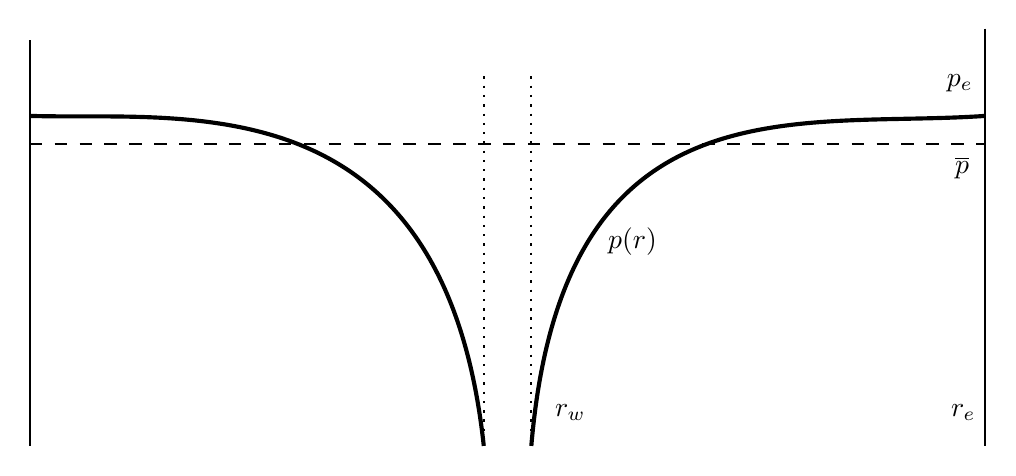
\begin{tikzpicture}[x=0.75pt,y=0.75pt,yscale=-1,xscale=1]
%uncomment if require: \path (0,300); %set diagram left start at 0, and has height of 300

%Curve Lines [id:da7511541250087521] 
\draw [line width=1.5]    (344.45,238) .. controls (359.67,59.33) and (472.6,85.33) .. (563.2,79) ;
%Curve Lines [id:da025905206061745956] 
\draw [line width=1.5]    (321.55,238) .. controls (302.33,60.67) and (177,81.33) .. (102.8,79) ;
%Straight Lines [id:da6790536850628852] 
\draw  [dash pattern={on 0.84pt off 2.51pt}]  (321.55,60) -- (321.55,238) ;
%Straight Lines [id:da4154351528354687] 
\draw  [dash pattern={on 0.84pt off 2.51pt}]  (344.45,60) -- (344.45,238) ;
%Straight Lines [id:da012417840094577581] 
\draw  [dash pattern={on 4.5pt off 4.5pt}]  (102.8,92.67) -- (563.2,92.67) ;
%Straight Lines [id:da923812897272561] 
\draw    (102.8,42.67) -- (102.8,238) ;
%Straight Lines [id:da9720690336089455] 
\draw    (563.2,37) -- (563.2,238) ;

% Text Node
\draw (354.45,216.4) node [anchor=north west][inner sep=0.75pt]    {$r_{w}$};
% Text Node
\draw (545.2,216.4) node [anchor=north west][inner sep=0.75pt]    {$r_{e}$};
% Text Node
\draw (543.2,57.4) node [anchor=north west][inner sep=0.75pt]    {$p_{e}$};
% Text Node
\draw (547.2,97.07) node [anchor=north west][inner sep=0.75pt]    {$\overline{p}$};
% Text Node
\draw (380,131.4) node [anchor=north west][inner sep=0.75pt]    {$p( r)$};


\end{tikzpicture}
		\caption{Схема радиального притока к скважине при наличии постоянного давления на границе}
		\label{ris:radial_inflow_steady_state_average_pressure}
	\end{center}
\end{figure}

В приведенное выражение входит значение давления на контуре, которым не всегда бывает удобно пользоваться. В практических случаях значение на контуре трудно оценить, контур зоны дренирования может значительно отличаться от кругового, да и радиус оценить может быть сложно. Удобнее пользоваться средним давлением в зоне дренирования $\bar{P}$, которое может быть оценено по материальному балансу (смотри рисунок \ref{ris:radial_inflow_steady_state_average_pressure}). 



%[[вывод уравнения фильтрации для постоянного давления на границе с использованием среднего давления]]
В этом случае выражение для дебита примет вид
$$q=\frac{kh\left( \bar{P}-P_w\right)}{ 18.41 \mu\left(\ln{\dfrac{r_e}{r_w}}  - \dfrac{1}{2}+ S \right)}$$


\subsection{Решение для круговой непроницаемой границы}

Схема модели радиального притока для условия непротекания на круговой границе приведена на рисунке \ref{ris:radial_inflow_steady_state_2}.

\begin{figure}[h!]
	\begin{center}
		

\tikzset{every picture/.style={line width=0.75pt}} %set default line width to 0.75pt        

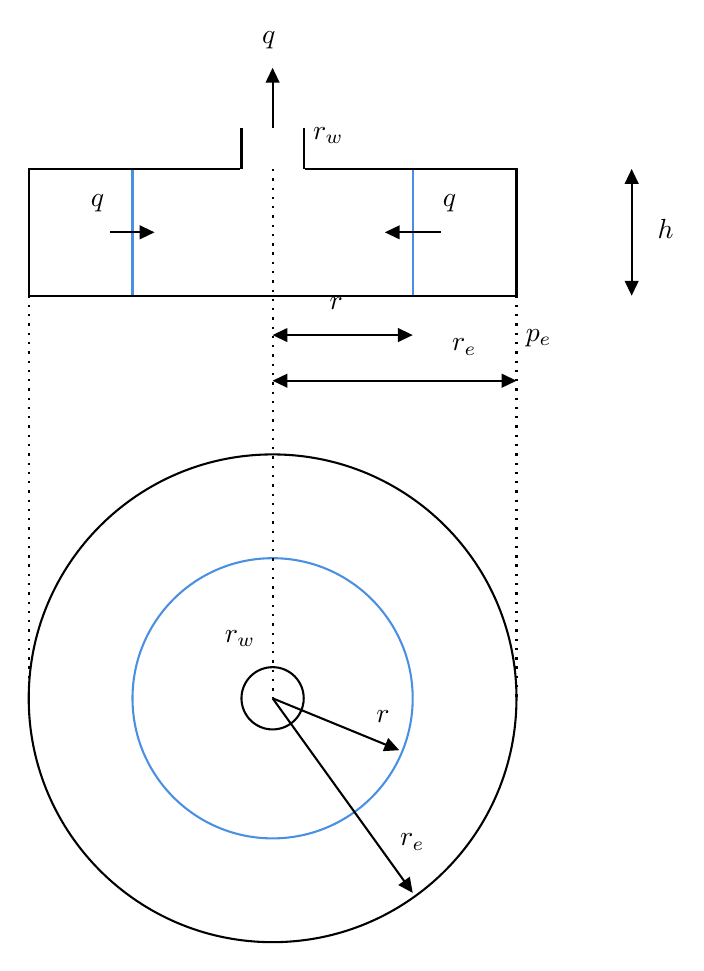
\begin{tikzpicture}[x=0.75pt,y=0.75pt,yscale=-1,xscale=1]
%uncomment if require: \path (0,542); %set diagram left start at 0, and has height of 542

%Shape: Rectangle [id:dp9986954540947564] 
\draw  [color={rgb, 255:red, 74; green, 144; blue, 226 }  ,draw opacity=1 ] (275.5,106.5) -- (410.5,106.5) -- (410.5,167.5) -- (275.5,167.5) -- cycle ;
%Shape: Circle [id:dp6552629065863149] 
\draw  [color={rgb, 255:red, 74; green, 144; blue, 226 }  ,draw opacity=1 ][fill={rgb, 255:red, 255; green, 255; blue, 255 }  ,fill opacity=1 ] (275.5,361.5) .. controls (275.5,324.22) and (305.72,294) .. (343,294) .. controls (380.28,294) and (410.5,324.22) .. (410.5,361.5) .. controls (410.5,398.78) and (380.28,429) .. (343,429) .. controls (305.72,429) and (275.5,398.78) .. (275.5,361.5) -- cycle ;
%Shape: Circle [id:dp8082105624253089] 
\draw   (225.5,361.5) .. controls (225.5,296.61) and (278.11,244) .. (343,244) .. controls (407.89,244) and (460.5,296.61) .. (460.5,361.5) .. controls (460.5,426.39) and (407.89,479) .. (343,479) .. controls (278.11,479) and (225.5,426.39) .. (225.5,361.5) -- cycle ;
%Shape: Rectangle [id:dp8805209935477971] 
\draw   (225.5,106.5) -- (460.5,106.5) -- (460.5,167.5) -- (225.5,167.5) -- cycle ;
%Shape: Rectangle [id:dp9848620821804102] 
\draw  [color={rgb, 255:red, 255; green, 255; blue, 255 }  ,draw opacity=1 ][fill={rgb, 255:red, 255; green, 255; blue, 255 }  ,fill opacity=1 ] (328,96) -- (358,96) -- (358,117) -- (328,117) -- cycle ;
%Shape: Circle [id:dp7806087558343378] 
\draw   (328,361.5) .. controls (328,353.22) and (334.72,346.5) .. (343,346.5) .. controls (351.28,346.5) and (358,353.22) .. (358,361.5) .. controls (358,369.78) and (351.28,376.5) .. (343,376.5) .. controls (334.72,376.5) and (328,369.78) .. (328,361.5) -- cycle ;
%Straight Lines [id:da7744729507427655] 
\draw  [dash pattern={on 0.84pt off 2.51pt}]  (225.5,167.5) -- (225.5,361.5) ;
%Straight Lines [id:da34517185100966685] 
\draw  [dash pattern={on 0.84pt off 2.51pt}]  (460.5,167.5) -- (460.5,361.5) ;
%Straight Lines [id:da3585865226685445] 
\draw    (328,86.5) -- (328,106.5) ;
%Straight Lines [id:da41145580018262384] 
\draw    (358,86.5) -- (358,106.5) ;
%Straight Lines [id:da4626155220696013] 
\draw  [dash pattern={on 0.84pt off 2.51pt}]  (343,106.5) -- (343,361.5) ;
%Straight Lines [id:da5723626081572117] 
\draw    (343,361.5) -- (408.75,452.82) ;
\draw [shift={(410.5,455.25)}, rotate = 234.25] [fill={rgb, 255:red, 0; green, 0; blue, 0 }  ][line width=0.08]  [draw opacity=0] (7.14,-3.43) -- (0,0) -- (7.14,3.43) -- cycle    ;
%Straight Lines [id:da9257805385062015] 
\draw    (343,361.5) -- (401.22,385.36) ;
\draw [shift={(404,386.5)}, rotate = 202.29] [fill={rgb, 255:red, 0; green, 0; blue, 0 }  ][line width=0.08]  [draw opacity=0] (7.14,-3.43) -- (0,0) -- (7.14,3.43) -- cycle    ;
%Straight Lines [id:da15606395599455936] 
\draw    (346,186.5) -- (407.5,186.5) ;
\draw [shift={(410.5,186.5)}, rotate = 180] [fill={rgb, 255:red, 0; green, 0; blue, 0 }  ][line width=0.08]  [draw opacity=0] (7.14,-3.43) -- (0,0) -- (7.14,3.43) -- cycle    ;
\draw [shift={(343,186.5)}, rotate = 0] [fill={rgb, 255:red, 0; green, 0; blue, 0 }  ][line width=0.08]  [draw opacity=0] (7.14,-3.43) -- (0,0) -- (7.14,3.43) -- cycle    ;
%Straight Lines [id:da6156171963471699] 
\draw    (346,208.5) -- (457.5,208.5) ;
\draw [shift={(460.5,208.5)}, rotate = 180] [fill={rgb, 255:red, 0; green, 0; blue, 0 }  ][line width=0.08]  [draw opacity=0] (7.14,-3.43) -- (0,0) -- (7.14,3.43) -- cycle    ;
\draw [shift={(343,208.5)}, rotate = 0] [fill={rgb, 255:red, 0; green, 0; blue, 0 }  ][line width=0.08]  [draw opacity=0] (7.14,-3.43) -- (0,0) -- (7.14,3.43) -- cycle    ;
%Straight Lines [id:da29225849394418124] 
\draw    (343,86.5) -- (343,60.75) ;
\draw [shift={(343,57.75)}, rotate = 450] [fill={rgb, 255:red, 0; green, 0; blue, 0 }  ][line width=0.08]  [draw opacity=0] (7.14,-3.43) -- (0,0) -- (7.14,3.43) -- cycle    ;
%Straight Lines [id:da05244651066444139] 
\draw    (264.9,137) -- (283.1,137) ;
\draw [shift={(286.1,137)}, rotate = 180] [fill={rgb, 255:red, 0; green, 0; blue, 0 }  ][line width=0.08]  [draw opacity=0] (7.14,-3.43) -- (0,0) -- (7.14,3.43) -- cycle    ;
%Straight Lines [id:da42364169594920353] 
\draw    (423.95,137) -- (400.1,137) ;
\draw [shift={(397.1,137)}, rotate = 360] [fill={rgb, 255:red, 0; green, 0; blue, 0 }  ][line width=0.08]  [draw opacity=0] (7.14,-3.43) -- (0,0) -- (7.14,3.43) -- cycle    ;
%Straight Lines [id:da523288490832504] 
\draw    (516,109.5) -- (516,164.5) ;
\draw [shift={(516,167.5)}, rotate = 270] [fill={rgb, 255:red, 0; green, 0; blue, 0 }  ][line width=0.08]  [draw opacity=0] (7.14,-3.43) -- (0,0) -- (7.14,3.43) -- cycle    ;
\draw [shift={(516,106.5)}, rotate = 90] [fill={rgb, 255:red, 0; green, 0; blue, 0 }  ][line width=0.08]  [draw opacity=0] (7.14,-3.43) -- (0,0) -- (7.14,3.43) -- cycle    ;

% Text Node
\draw (336.5,38.9) node [anchor=north west][inner sep=0.75pt]    {$q$};
% Text Node
\draw (361,84.9) node [anchor=north west][inner sep=0.75pt]    {$r_{w}$};
% Text Node
\draw (254,117.4) node [anchor=north west][inner sep=0.75pt]    {$q$};
% Text Node
\draw (423.5,117.4) node [anchor=north west][inner sep=0.75pt]    {$q$};
% Text Node
\draw (369,166.9) node [anchor=north west][inner sep=0.75pt]    {$r$};
% Text Node
\draw (428,186.9) node [anchor=north west][inner sep=0.75pt]    {$r_{e}$};
% Text Node
\draw (318.5,327.4) node [anchor=north west][inner sep=0.75pt]    {$r_{w}$};
% Text Node
\draw (391.5,365.9) node [anchor=north west][inner sep=0.75pt]    {$r$};
% Text Node
\draw (403,425.4) node [anchor=north west][inner sep=0.75pt]    {$r_{e}$};
% Text Node
\draw (463.5,182.4) node [anchor=north west][inner sep=0.75pt]    {$p_{e}$};
% Text Node
\draw (527,129.4) node [anchor=north west][inner sep=0.75pt]    {$h$};


\end{tikzpicture}
		\caption{Схема радиального притока к скважине при наличии непроницаемой границы}
		\label{ris:radial_inflow_steady_state_2}
	\end{center}
\end{figure}

При условии непротекания давления на границе условия стационарности (неизменности давления) не достигаются. При работе скважины с постоянным дебитом забойное давление будет постоянно снижаться. Однако начиная с некоторого момента, когда влияние скважины достигнет границ - давление в всей области дренирования начнет снижаться равномерно (смотри рисунок \ref{ris:radial_pss_dynamics}). 

\begin{figure}[h!]
	\begin{center}
		

\tikzset{every picture/.style={line width=0.75pt}} %set default line width to 0.75pt        

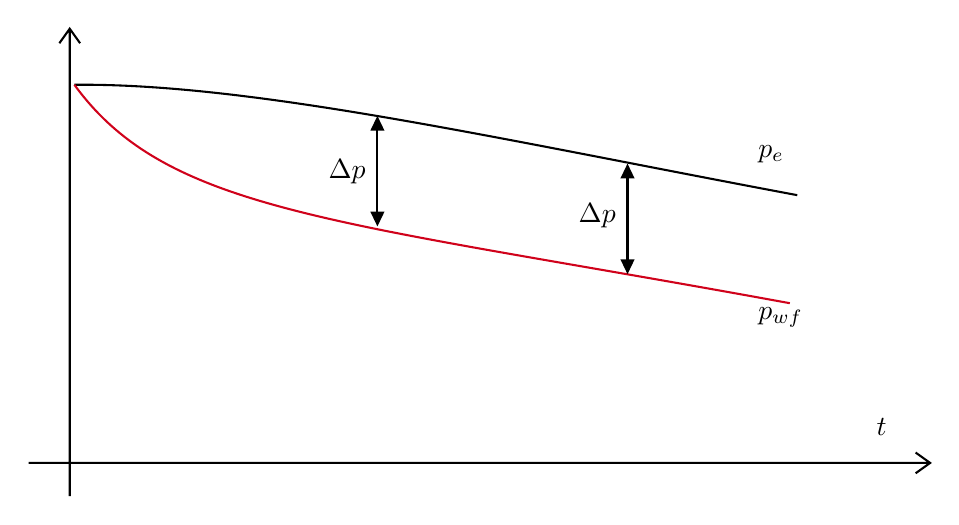
\begin{tikzpicture}[x=0.75pt,y=0.75pt,yscale=-1,xscale=1]
%uncomment if require: \path (0,300); %set diagram left start at 0, and has height of 300

%Shape: Axis 2D [id:dp9842834583970732] 
\draw  (121,262.2) -- (555.3,262.2)(140.76,53) -- (140.76,278.2) (548.3,257.2) -- (555.3,262.2) -- (548.3,267.2) (135.76,60) -- (140.76,53) -- (145.76,60)  ;
%Curve Lines [id:da6767694694353563] 
\draw    (143,80) .. controls (229.3,79.2) and (347.3,106.2) .. (491.3,133.2) ;
%Curve Lines [id:da1513616030724707] 
\draw [color={rgb, 255:red, 208; green, 2; blue, 27 }  ,draw opacity=1 ]   (143,80) .. controls (188.3,142.2) and (269.7,145.25) .. (487.7,185.25) ;
%Straight Lines [id:da13598982031442275] 
\draw    (289,98) -- (289,145.25) ;
\draw [shift={(289,148.25)}, rotate = 270] [fill={rgb, 255:red, 0; green, 0; blue, 0 }  ][line width=0.08]  [draw opacity=0] (7.14,-3.43) -- (0,0) -- (7.14,3.43) -- cycle    ;
\draw [shift={(289,95)}, rotate = 90] [fill={rgb, 255:red, 0; green, 0; blue, 0 }  ][line width=0.08]  [draw opacity=0] (7.14,-3.43) -- (0,0) -- (7.14,3.43) -- cycle    ;
%Straight Lines [id:da13673864754675735] 
\draw    (409.5,121) -- (409.5,168.25) ;
\draw [shift={(409.5,171.25)}, rotate = 270] [fill={rgb, 255:red, 0; green, 0; blue, 0 }  ][line width=0.08]  [draw opacity=0] (7.14,-3.43) -- (0,0) -- (7.14,3.43) -- cycle    ;
\draw [shift={(409.5,118)}, rotate = 90] [fill={rgb, 255:red, 0; green, 0; blue, 0 }  ][line width=0.08]  [draw opacity=0] (7.14,-3.43) -- (0,0) -- (7.14,3.43) -- cycle    ;

% Text Node
\draw (264,114.4) node [anchor=north west][inner sep=0.75pt]    {$\Delta p$};
% Text Node
\draw (384.5,135.9) node [anchor=north west][inner sep=0.75pt]    {$\Delta p$};
% Text Node
\draw (471,107.9) node [anchor=north west][inner sep=0.75pt]    {$p_{e}$};
% Text Node
\draw (471,185.9) node [anchor=north west][inner sep=0.75pt]    {$p_{wf}$};
% Text Node
\draw (528,239.4) node [anchor=north west][inner sep=0.75pt]    {$t$};


\end{tikzpicture}
		\caption{Изменение давления на границе и на забое скважины во времени}
		\label{ris:radial_pss_dynamics}
	\end{center}
\end{figure}

Такой режим, при котором забойное давление меняется, но перепад давления $P_e - P_w$ остается постоянным называют псевдо-установившимся режимом работы (pss - pseudo steady state). 

Для псевдо-установившегося режима можно записать выражение

$$q=\frac{kh\left(P_e-P_w\right)}{ 18.41 \mu\left(\ln{\dfrac{r_e}{r_w}} - \dfrac{1}{2} + S\right)}$$
где 

$q$ - объемные дебит скважины в рабочих условиях, м3/сут;

$r$ -  радиус - расстояние от центра скважины, м;

$r_e$ -  радиус зоны дренирования, на котором поддерживается постоянное давление, м;

$r_w$ - радиус скважины, на котором замеряется забойное давление, м;

$P$ - давление, атм;

$P_e$ - давление на внешнем контуре дренирования, атм;

$P_w$ - давление на забое скважины, атм;

$k$ - проницаемость, мД;

$\mu$ - вязкость нефти в зоне дренирования, сП.

\

\subsection{Решение для круговой непроницаемой границы с учетом среднего давления в зоне дренирования}

Аналогично случаю для постоянного давления на границе можно переписать выражение с использованием среднего давления в области дренирования. 

$$q=\frac{kh\left( \bar{P}-P_w\right)}{ 18.41 \mu\left(\ln{\dfrac{r_e}{r_w}} - \dfrac{3}{4}+ S \right)}$$

%[[Вывод уравнений для псевдо-установившегося режима работы]]



\subsection{Стационарные решения для вертикальной скважины в резервуаре произвольной формы}

Здесь уравнения и методы расчета для горизонтальных, наклонно направленных скважин, скважин с ГРП, горизонтальных скважин с МГРП. 

\begin{equation}
	q=\frac{kh\left( \bar{P}-P_w\right)}{ 18.41 \mu\left(\ln{\dfrac{2.2458 A}{C_A r_w^2}} + S \right)}
\end{equation}

$q$ - объемные дебит скважины в рабочих условиях, м3/сут;

$A$ -  площадь области дренирования, м$^2$;

$C_A$ -  фактор формы, зависит от формы резервуара и расположения скважины;

$r_w$ - радиус скважины, на котором замеряется забойное давление, м;

$\bar{P}$ - среднее давление в области дренирования, атм;

$P_e$ - давление на внешнем контуре дренирования, атм;

$P_w$ - давление на забое скважины, атм;

$k$ - проницаемость, мД;

$\mu$ - вязкость нефти в зоне дренирования, сП.

\

\begin{figure}[h!]
	\centering
	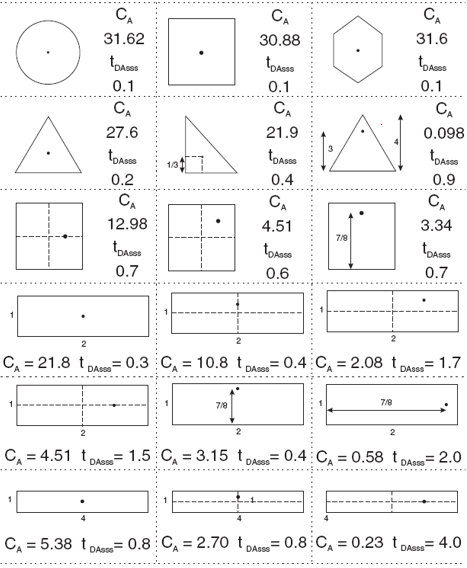
\includegraphics[width= 10cm]{pics/shape_factors.png} 
	\label{fig:shape_factors}
	\caption{Значения фактора формы}
\end{figure}

%todo -надо переделать рисунок и добавить ссылки на источники

Безразмерное время достижения псевдо-установившегося режима притока, определяемое видом резервуара

$$t_{DApss} = \frac{kt_{pss}}{\varphi \mu c_t A} $$

\subsection{Стационарные решения для скважины с трещиной ГРП}

%todo надо расписать четче и привести решение и для трещины конечной проводимости
Для больших времен скважину с трещиной ГРП можно представить как скважину с увеличенным "эффективным радиусом" $r_{eff}$, или, что эквивалентно, как скважину с отрицательным скин-фактором.

\begin{equation}
	r_{eff} = r_w e^{-S}
\end{equation}

Это верно, только если $x_f << r_e$

Для трещины бесконечной проводимости 

\begin{equation}
	r_{eff} = \frac{x_f}{2}
\end{equation}

тогда 

\begin{equation}
	S = \frac{2r_w}{x_f}
\end{equation}




